% Squares of sides F_1,...,F_5 tile an F_5 by F_6 rectangle.
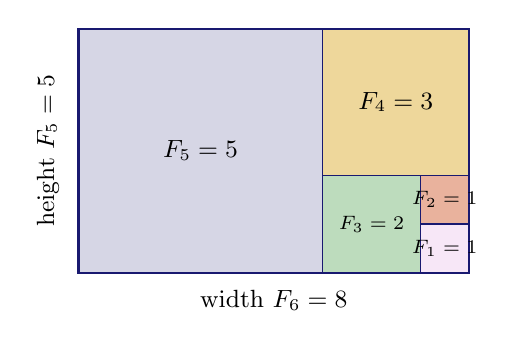
\begin{tikzpicture}[scale=0.62]
  \fill[MidnightBlue!18] (0,0) rectangle (5,5);
  \fill[Goldenrod!45] (5,2) rectangle (8,5);
  \fill[ForestGreen!30] (5,0) rectangle (7,2);
  \fill[BrickRed!28] (7,1) rectangle (8,2);
  \fill[Plum!25] (7,0) rectangle (8,1);
  \draw[MidnightBlue,thick] (0,0) rectangle (8,5);
  \draw[MidnightBlue] (5,0) -- (5,5);
  \draw[MidnightBlue] (5,2) -- (8,2);
  \draw[MidnightBlue] (7,0) -- (7,2);
  \draw[MidnightBlue] (7,1) -- (8,1);
  \node[font=\small] at (2.5,2.5) {$F_5=5$};
  \node[font=\small] at (6.5,3.5) {$F_4=3$};
  \node[font=\scriptsize] at (6.0,1.0) {$F_3=2$};
  \node[font=\scriptsize] at (7.5,1.5) {$F_2=1$};
  \node[font=\scriptsize] at (7.5,0.5) {$F_1=1$};
  \node[font=\small,below] at (4,-0.15) {width $F_6=8$};
  \node[font=\small,rotate=90,anchor=south] at (-0.2,2.5) {height $F_5=5$};
\end{tikzpicture}
